\documentclass[11pt, a4paper]{article}
\usepackage[top=3cm,bottom=3cm,left=2.75cm,right=2cm]{geometry}
\usepackage{graphicx} 
\usepackage[latin1]{inputenc}
\usepackage[spanish]{babel}
\usepackage{amsmath}

\begin{document}


\begin{figure}[t] %[h] para here [b] para bottom [t] para top
\centering

\includegraphics[width=80pt]{./logo.jpg}
\end{figure}


\begin{center}


\LARGE{UNIVERSIDAD DE BUENOS AIRES}
\Large{FACULTAD DE CIENCIAS EXACTAS Y NATURALES\\
DEPARTAMENTO DE COMPUTACI\'ON\\
\vspace{1.5cm}
ORGANIZACI\'ON DEL COMPUTADOR II\\
Segundo Cuatrimestre de 2009}

\vskip 50pt
\textbf{\Large{Procesamiento de Im\'agenes para la Detecci\'on de Bordes}}

\end{center}

\vskip 30pt

\begin{center}
\begin{tabular}{|lcl|}
\hline Integrante  & LU & Correo electr\'onico \\ 
\hline Bianchi, Mariano &  92/08 & \texttt{bianchi-mariano@hotmail.com}\\ 
Brusco, Pablo & 527/08 & \texttt{pablo.brusco@gmail.com} \\ 
Di Pietro, Carlos Augusto Lyon & 126/08 & \texttt{cdipietro@dc.uba.ar}\\ 
\hline 
\end{tabular} 

\vspace{20 pt}

Grupo : PUNPCKHQDQ

\end{center}

\vskip 60pt

{\small
\flushleft{\textbf{Resumen}}\\
La detecci\'on de bordes es una herramienta sumamente utilizada en el procesamiento de im\'agenes, la cual permite dar mayor importancia a ciertos datos como son las l\'neas, los contornos y trazos de las mismas en detrimento de otros detalles como pueden ser matices sutiles y l\'ineas muy finas. La idea del presente trabajo es lograr implementar algoritmos de detecci\'on de bordes de im\'agenes vali\'endose para ello de los operadores m\'as comunes para tal fin. Estos son los operadores de Sobel, Prewitt y Roberts.\\ 
Como paso ulterior se buscar\'a comparar los resultados obtenidos con funciones an\'alogas implementadas en la librer\'ia estandar de c\'odigo abierto OpenCV. Los aspectos a comparar ser\'an tanto la calidad de resultados como el tiempo de 
procesamiento medido en ciclos de reloj.\\

\vspace{22 pt}

\flushleft{\textbf{Palabras clave}}\\
Deteccion de bordes, Sobel, Roberts, Prewitt, convoluci\'on, imagenes, Lena , OpenCV.
}


\newpage

\section{Introducci\'on}


\newpage

\section{Desarrollo}


\newpage

\section{Resultados}


\newpage

\section{Debate}


\newpage

\section{Conclusi\'on}



\newpage
\section{Anexo I}
\subsection{Imagenes resultantes del procesamiento de detecci\'on de bordes}

\vspace{2cm}

\begin{figure}[ht] %[h] para here [b] para bottom [t] para top
\centering
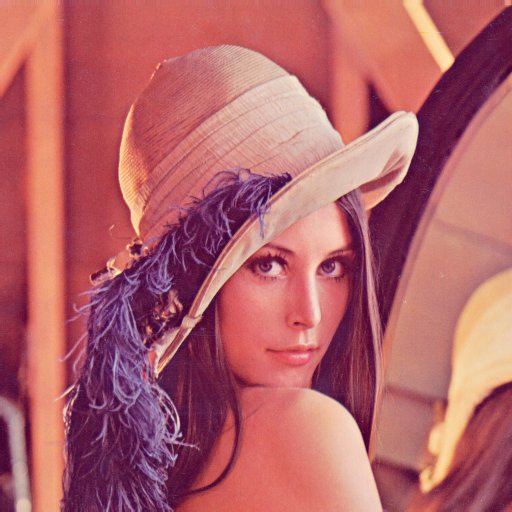
\includegraphics[scale=0.25]{lena.bmp}
\caption{Primer imagen utilizada para detecci\'on de bordes - lena.jpg}
\end{figure}


\end{document}
